	
% This template from http://www.vel.co.nz, originally from http://www.tedpavlic.com

\documentclass{article}
% Change "article" to "report" to get rid of page number on title page
\usepackage{amsmath,amsfonts,amsthm,amssymb, mathrsfs}
\usepackage{bigints}
\usepackage{setspace}
\usepackage{Tabbing}
\usepackage{fancyhdr}
\usepackage{lastpage}
\usepackage{textcomp}
\usepackage{extramarks}
\usepackage{chngpage}
\usepackage{soul,color}
\usepackage{graphicx,float,wrapfig}
\usepackage{cancel}
\usepackage{indentfirst}
\usepackage{mdframed}

% In case you need to adjust margins:
\topmargin=-0.45in      %
\evensidemargin=0in     %
\oddsidemargin=0in      %
\textwidth=6.5in        %
\textheight=9.0in       %
\headsep=0.25in         %

% Homework Specific Information
\newcommand{\hmwkTitle}{WS3}
\newcommand{\hmwkDueDate}{}
\newcommand{\hmwkClass}{Ay\ 190}
\newcommand{\hmwkAuthorName}{Cutter\ Coryell}

% Setup the header and footer
\pagestyle{fancy}                                                       %
\lhead{\hmwkAuthorName}                                                 %
\chead{\hmwkClass\ : \hmwkTitle}  %
\rhead{\hmwkDueDate}                                                     %
\renewcommand\headrulewidth{0.4pt}                                      %
\renewcommand\footrulewidth{0.4pt}                                      %

% This is used to trace down (pin point) problems
% in latexing a document:
%\tracingall

%%%%%%%%%%%%%%%%%%%%%%%%%%%%%%%%%%%%%%%%%%%%%%%%%%%%%%%%%%%%%
% Some tools
\newcommand{\enterProblemHeader}[1]{\nobreak\extramarks{#1}{#1 continued on next page\ldots}\nobreak%
                                    \nobreak\extramarks{#1 (continued)}{#1 continued on next page\ldots}\nobreak}%
\newcommand{\exitProblemHeader}[1]{\nobreak\extramarks{#1 (continued)}{#1 continued on next page\ldots}\nobreak%
                                   \nobreak\extramarks{#1}{}\nobreak}%

\newlength{\labelLength}
\newcommand{\labelAnswer}[2]
  {\settowidth{\labelLength}{#1}%
   \addtolength{\labelLength}{0.25in}%
   \changetext{}{-\labelLength}{}{}{}%
   \noindent\fbox{\begin{minipage}[c]{\columnwidth}#2\end{minipage}}%
   \marginpar{\fbox{#1}}%

   % We put the blank space above in order to make sure this
   % \marginpar gets correctly placed.
   \changetext{}{+\labelLength}{}{}{}}%

\setcounter{secnumdepth}{0}
\newcommand{\homeworkProblemName}{}%
\newcounter{homeworkProblemCounter}%
\newenvironment{homeworkProblem}[1][Problem \arabic{homeworkProblemCounter}]%
  {\stepcounter{homeworkProblemCounter}%
   \renewcommand{\homeworkProblemName}{#1}%
   \section{\homeworkProblemName}%
   \enterProblemHeader{\homeworkProblemName}}%
  {\exitProblemHeader{\homeworkProblemName}}%

\newcommand{\problemAnswer}[1]
  {\noindent\fbox{\begin{minipage}[c]{\columnwidth}#1\end{minipage}}}%

\newcommand{\problemLAnswer}[1]
  {\labelAnswer{\homeworkProblemName}{#1}}

\newcommand{\homeworkSectionName}{}%
\newlength{\homeworkSectionLabelLength}{}%
\newenvironment{homeworkSection}[1]%
  {% We put this space here to make sure we're not connected to the above.
   % Otherwise the changetext can do funny things to the other margin

   \renewcommand{\homeworkSectionName}{#1}%
   \settowidth{\homeworkSectionLabelLength}{\homeworkSectionName}%
   \addtolength{\homeworkSectionLabelLength}{0.25in}%
   \changetext{}{-\homeworkSectionLabelLength}{}{}{}%
   \subsection{\homeworkSectionName}%
   \enterProblemHeader{\homeworkProblemName\ [\homeworkSectionName]}}%
  {\enterProblemHeader{\homeworkProblemName}%

   % We put the blank space above in order to make sure this margin
   % change doesn't happen too soon (otherwise \sectionAnswer's can
   % get ugly about their \marginpar placement.
   \changetext{}{+\homeworkSectionLabelLength}{}{}{}}%

\newcommand{\sectionAnswer}[1]
  {% We put this space here to make sure we're disconnected from the previous
   % passage

   \noindent\fbox{\begin{minipage}[c]{\columnwidth}#1\end{minipage}}%
   \enterProblemHeader{\homeworkProblemName}\exitProblemHeader{\homeworkProblemName}%
   \marginpar{\fbox{\homeworkSectionName}}%

   % We put the blank space above in order to make sure this
   % \marginpar gets correctly placed.
   }%

\newenvironment{myindentpar}[1]%
 {\begin{list}{}%
         {\setlength{\leftmargin}{#1}}%
         \item[]%
 }
 {\end{list}}

%%%%%%%%%%%%%%%%%%%%%%%%%%%%%%%%%%%%%%%%%%%%%%%%%%%%%%%%%%%%%


%%%%%%%%%%%%%%%%%%%%%%%%%%%%%%%%%%%%%%%%%%%%%%%%%%%%%%%%%%%%%
% Make title
\title{\vspace{2in}\textmd{\textbf{\hmwkClass:\ \hmwkTitle}}\\\normalsize\vspace{0.1in}\small{Due\ on\ \hmwkDueDate}\\\vspace{0.1in}\large{\textit{\hmwkClassInstructor\ \hmwkClassTime}}\vspace{3in}}
\date{}
\author{\textbf{\hmwkAuthorName}}
%%%%%%%%%%%%%%%%%%%%%%%%%%%%%%%%%%%%%%%%%%%%%%%%%%%%%%%%%%%%%

%%%% MY COMMANDS %%%%%%%%%%%%%%%%%%%%%

\newcommand{\deri}[2]{\frac{\mathrm{d} #1}{\mathrm{d} #2}}
\newcommand{\pderi}[2]{\frac{\partial #1}{\partial #2}}
\newcommand{\inte}[4]{\int_{#1}^{#2} \! #3 \, \mathrm{d} #4}
\newcommand{\ointe}[4]{\oint_{#1}^{#2} \! #3 \, \mathrm{d} #4}
\newcommand{\del}{\nabla}
\newcommand{\D}{\mathrm{d}}
\newcommand{\ee}[1]{\times 10^{#1}}
\newcommand{\fpe}{\frac{1}{4 \pi \epsilon_0}}
\newcommand{\bra}[1]{\left< #1 \right|}
\newcommand{\ket}[1]{\left| #1 \right>}
\newcommand{\cket}[1]{\left. #1 \right>}


% Distance units
\newcommand{\m}[0]{\text{\ m}}
\newcommand{\cm}[0]{\text{\ cm}}
\newcommand{\km}[0]{\text{\ km}}
\newcommand{\pc}[0]{\text{\ pc}}
\newcommand{\kpc}[0]{\text{\ kpc}}
\newcommand{\Mpc}[0]{\text{\ Mpc}}
\newcommand{\Gpc}[0]{\text{\ Gpc}}
\newcommand{\lyr}[0]{\text{\ lyr}}
\newcommand{\Rs}[0]{R_\odot}

% Mass units
\newcommand{\g}[0]{\text{\ g}}
\newcommand{\kg}[0]{\text{\ kg}}
\newcommand{\Ms}[0]{M_\odot}

% Time units
\newcommand{\s}[0]{\text{\ s}}
\newcommand{\days}[0]{\text{\ days}}
\newcommand{\yr}[0]{\text{\ yr}}
\newcommand{\Hz}[0]{\text{\ Hz}}
\newcommand{\kHz}[0]{\text{\ kHz}}
\newcommand{\MHz}[0]{\text{\ MHz}}
\newcommand{\GHz}[0]{\text{\ GHz}}
\newcommand{\THz}[0]{\text{\ THz}}

% Energy units
\newcommand{\erg}[0]{\text{\ erg}}
\newcommand{\J}[0]{\text{\ J}}
\newcommand{\eV}[0]{\text{\ eV}}
\newcommand{\meV}[0]{\text{\ meV}}
\newcommand{\keV}[0]{\text{\ keV}}
\newcommand{\MeV}[0]{\text{\ MeV}}
\newcommand{\GeV}[0]{\text{\ GeV}}
\newcommand{\TeV}[0]{\text{\ TeV}}

% Force units
\newcommand{\N}[0]{\text{\ N}}
\newcommand{\dyn}[0]{\text{\ dyn}}

% Power units
\newcommand{\W}[0]{\text{\ W}}
\newcommand{\Ls}[0]{L_\odot}

% Temperature units
\newcommand{\K}[0]{\text{\ K}}
\newcommand{\degC}[0]{\text{\ \(^\circ\)C}}
\newcommand{\degF}[0]{\text{\ \(^\circ\)F}}

% Electromagnetic units
\newcommand{\V}[0]{\text{\ V}}
\newcommand{\kV}[0]{\text{\ kV}}
\newcommand{\C}[0]{\text{\ C}}
\newcommand{\esu}[0]{\text{\ esu}}
\newcommand{\T}[0]{\text{\ T}}
\newcommand{\G}[0]{\text{\ G}}


\newcount\colveccount
\newcommand*\colvec[1]{
        \global\colveccount#1
        \begin{pmatrix}
        \colvecnext
}
\def\colvecnext#1{
        #1
        \global\advance\colveccount-1
        \ifnum\colveccount>0
                \\
                \expandafter\colvecnext
        \else
                \end{pmatrix}
        \fi
}

%%%%%%%%%%%%%%%%%%%%%%%%%%%%%%%%%%

\begin{document}
\begin{spacing}{1.1}

\newpage

% When problems are long, it may be desirable to put a \newpage or a
% \clearpage before each homeworkProblem environment

I worked with David Vartanyan (my partner) and John Pharo on this worksheet. It took about five hours total time.

\subsection{1. Integration via Newton-Cotes Formulae }

\subsubsection{Part A}

I computed \(\inte{0}{\pi}{\sin x}{x}\) via the Midpoint, Trapezoidal, and Simpson's Approximations. The analytical answer is 2. Errors and convergence orders are presented below. \\

\noindent Relative errors in approximations at 100 grid points: \\ \\
    \begin{tabular}{lr}
	Midpoint & \(4.19595546677\ee{-5}\) \\
	Trapezoidal &	 \(-8.39180530038\ee{-5} \)\\
	Simpson's &	 \(3.52111007018\ee{-10}\)\\

	\end{tabular} \\ \\

\noindent Convergence order (\(\log_2\) of the factor decrease in error size when resolution is doubled): \\ \\
\begin{tabular}{lrr}
Midpoint 	& 2.01456788742 & (should be 1) \\
Trapezoidal &	 2.01455422188 & (should be 2) \\
Simpson's 	& 4.02909033045 & (should be 4) \\
\end{tabular} \\ \\

The Midpoint Approximation has comparable error to the Trapezoidal Approximation; in fact it has one half the error to 4 sig-figs, which is an extremely strange coincidence. It makes sense that these errors should be comparable; it was pointed out in lecture that the Midpoint Approximation "cheats" by having part of the line higher above the function curve and part below, thus canceling error. That said, I do not know why the Midpoint Approximation has a higher convergence order than it should (it should be globally first-order), despite careful inspection of my implementation. It is strange that the convergence order is so close to that of the Trapezoidal Approximation.

\subsubsection{Part B}

I computed \(\inte{0}{\pi}{x \sin x}{x}\) via the Midpoint, Trapezoidal, and Simpson's Approximations. The analytical answer is \(\pi\). Errors and convergence orders are presented below. \\

\noindent Relative errors in approximations at 100 grid points: \\ \\
    \begin{tabular}{lr}
	Midpoint & \(4.19595546682\ee{-5}\) \\
	Trapezoidal &	 \(-8.39180530038\ee{-5} \)\\
	Simpson's &	 \(3.5211044459\ee{-10}\)\\

	\end{tabular} \\ \\

\noindent Convergence order (\(\log_2\) of the factor decrease in error size when resolution is doubled): \\ \\
\begin{tabular}{lrr}
Midpoint 	& 2.0145678874 & (should be 1) \\
Trapezoidal &	 2.01455422188 & (should be 2) \\
Simpson's 	& 4.02905577134 & (should be 4) \\
\end{tabular} \\ \\

Again, I do not know why the Midpoint Approximation has a higher convergence order than it should. Also curious is that my relative errors and convergence orders are almost exactly the same between the two integrands in Parts A and B.

\newpage
\subsection{2. Gaussian Quadrature}

\subsubsection{Part A}

First we calculate the coefficient to the integral in Eq. 1:

\[
\frac{8 \pi \left(k_B T\right)^3}{\left(2 \pi \hbar c\right)^3} = 1.05495\ee{35} \cm^{-3}
\]

We set the weight function \(W(x) = e^{-x}\) and the function \(f(x) = \frac{x^2 e^{x}}{e^x + 1}\). The resulting integrated number density is shown in Table~1 for various numbers of nodes in the Gauss-Laguerre Quadrature.

\begin{table}[H]
	\label{table1}
	\centering
    \begin{tabular}{|c|c|c|}
	\hline
	
	Number of nodes \(n\) & Number density \([\cm^{-3}]\) & Change in number density \([\cm^{-3}]\) \\

	\hline

    2 & \(1.22842960\ee{31}\) & - \\
    4 & \(6.03420893\ee{32}\) & \(5.91136597\ee{32}\) \\ 
    8 & \(2.15112647\ee{34}\) & \(2.09078438\ee{34}\) \\
    16 & \(1.65635419\ee{35}\) & \(1.44124154\ee{35}\) \\
    32 & \(1.90216416\ee{35}\) & \(2.45809969\ee{34}\) \\
    64 & \(1.90216489\ee{35}\) & \(7.34916308\ee{28}\) \\
    128 & \(1.90216489\ee{35}\) & \(0.00000000\ee{0}\) \\
    
	\hline
	\end{tabular}
	\caption{Approximations to the number density integral of Eq. 1 using the Gauss-Laguerre Quadrature for various numbers of nodes \(n\). Also shown is the change in this approximation as \(n\) is varied, demonstrating convergence as this change vanishes for large \(n\).}
	\end{table}

\subsubsection{Part B}

Now we must transform the integral \(\inte{a}{b}{x^2 (e^x + 1)^{-1}}{x}\) such that it is over the interval [-1,1]. To do this, let \(y = \frac{2}{b-a} (x-a) - 1\). Then

\[
x(y) = (y + a) \frac{b-a}{2} + a
\]
\[
\inte{a}{b}{\frac{x^2}{e^x + 1}}{x} = \frac{b-a}{2}\inte{-1}{1}{\frac{x(y)^2}{e^{x(y)} + 1}}{y}
\]
This can then be computed with Gauss-Legendre Quadrature. The resulting number densities in each energy bin is depicted in Fig~\ref{fig2}. The sum of the number densities in each bin is \(1.85943561534\ee{35} \cm^{-3}\), which is slightly less than the converged answer from Part A of \(1.90216489\ee{35} \cm^{-3}\). However, this answer for Part B is invariant to decreasing energy bin width, increasing energy of maximum energy bin, and increasing the number of nodes for each bin's integration. Therefore there is an unknown systematic reason for this 2\% discrepancy.

\begin{figure}[H]
 \label{fig2}
 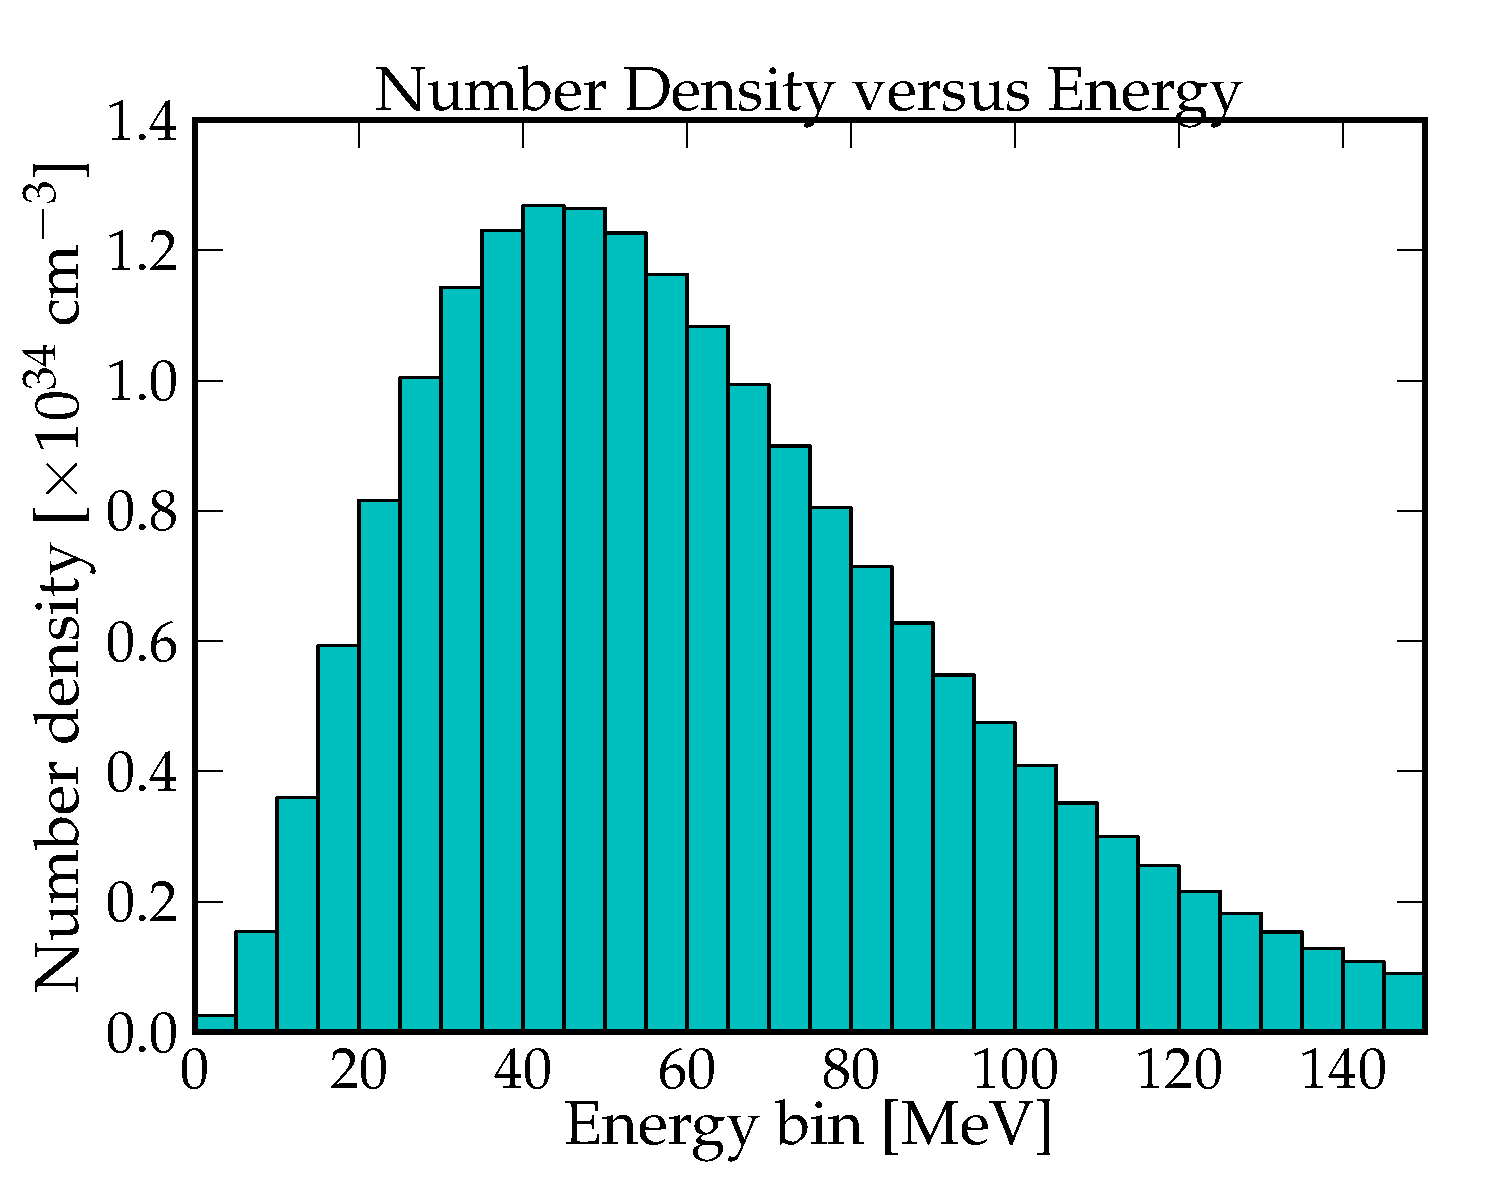
\includegraphics[width=\textwidth]{problem2b.pdf}
 \caption{A plot of the number densities of electrons and neutrinos in equilibrium with photons at a temperature of 20\MeV, separated into energy bins of 5\MeV width.}
\end{figure}

\end{spacing}
\end{document}

%%%%%%%%%%%%%%%%%%%%%%%%%%%%%%%%%%%%%%%%%%%%%%%%%%%%%%%%%%%%%
